\documentclass[article,colorback,accentcolor=tud4c, 11pt]{tudreport}
%\usepackage{ngerman}

\usepackage[stable]{footmisc}
\usepackage[ngerman]{hyperref}

\usepackage{longtable}
\usepackage{multirow}
\usepackage{booktabs}
\usepackage[utf8]{inputenc}
\usepackage[export]{adjustbox}
\graphicspath{ {screens/} }

\hypersetup{%
  pdftitle={TUD Corporate-Design f"ur {\LaTeX}},
  pdfauthor={C. v. Loewenich und J. Werner},
  pdfsubject={Beispieltext},
  pdfview=FitH,
  pdfstartview=FitV
}

\setcounter{seclinedepth}{1}

%%% Zum Tester der Marginalien %%%
  \newif\ifTUDmargin\TUDmarginfalse
  %%% Wird der Folgende Zeile einkommentiert,
  %%% werden Marginalien gesetzt.
  % \TUDmargintrue
  \ifTUDmargin\makeatletter
    \TUD@setmarginpar{2}
  \makeatother\fi
%%% ENDE: Zum Tester der Marginalien %%%

\newlength{\longtablewidth}
\setlength{\longtablewidth}{0.7\linewidth}
\addtolength{\longtablewidth}{-\marginparsep}
\addtolength{\longtablewidth}{-\marginparwidth}


% \settitlepicture{tudreport-pic}
% \printpicturesize

\title{Internet Praktikum of Telecooperation Group - Winter Term 2018/2019\\
	Project Topic: Interactive Door Panel for Office Availability\\ Team Foxtrot}
\subtitle{Artem Vopilov (email: mister.0026@yandex.ru)\\Florian Schunk (email: florian.schunk@stud.tu-darmstadt.de)\\ Javier Ochoa Serna (email: jochoaserna@hotmail.com)\\
	Pramod Pramod (email: pramod.pramod@stud.tu-darmstadt.de) \\ Frank Langoulant (email: fl1001@rbg.informatik.tu-darmstadt.de)}
%\setinstitutionlogo[width]{TUD_sublogo}
\uppertitleback{(\textaccent{\textbackslash uppertitleback})}
\lowertitleback{(\textaccent{\textbackslash lowertitleback})\hfill\today}
\institution{Telecooperation Group\\
	S2|02 A114
	Hochschulstraße 10
	64289 Darmstadt}
%\dedication{Hier ist gen"ugend Platz\\
%  f"ur eine Widmung (\textaccent{\textbackslash dedication}).\\
%  \strut\\
%  F"ur Annelore Schmidt\\
%  aus dem Referat Kommunikation.\\
%  Sie hat immer ein offenes Ohr\\
%  f"ur unsere Fragen und Anregungen.}


\begin{document}
	\maketitle
	\begin{abstract}
		In this project we implement a doorpanel application designed to run on  Android Tablet as well as the counterpart application designed to run on android smartphones. The intention is to display information about the office room the doorpanel is assigned to as well as the workers in this office and their availability status. If the workers don't want to be disturbed by visitors comming by, the application provides the means to request an appointment as well as to send a message to a worker.
	\end{abstract}  
	
	\tableofcontents
	%%\part{Lorem Ipsum (\textbackslash part)\label{part_lorem}}
	\newpage
	
	\section{Motivation}
	
Traditional doorpanel signes printed on paper may be quite common but they lack a lot of possibilities. Every time there is a change cencerning the workers assigned to the office room, the sign needs to be reprinted and replaced. Even more important, the workers have no means to indicate to visitors passing by and maybe wanting to talk to a worker inside the office if they are welcome to enter or if a disturbance is currently inappropriate.

In order to change that we implemented an interactive doorpanel application to meet the requirements of up to date offices and their personel. 


	\section{Structure}
	Lorem ipsum  
	
	
	\subsection{Structural Overview}
	Lorem ipsum
	 \begin{figure}
	   %\centering
	   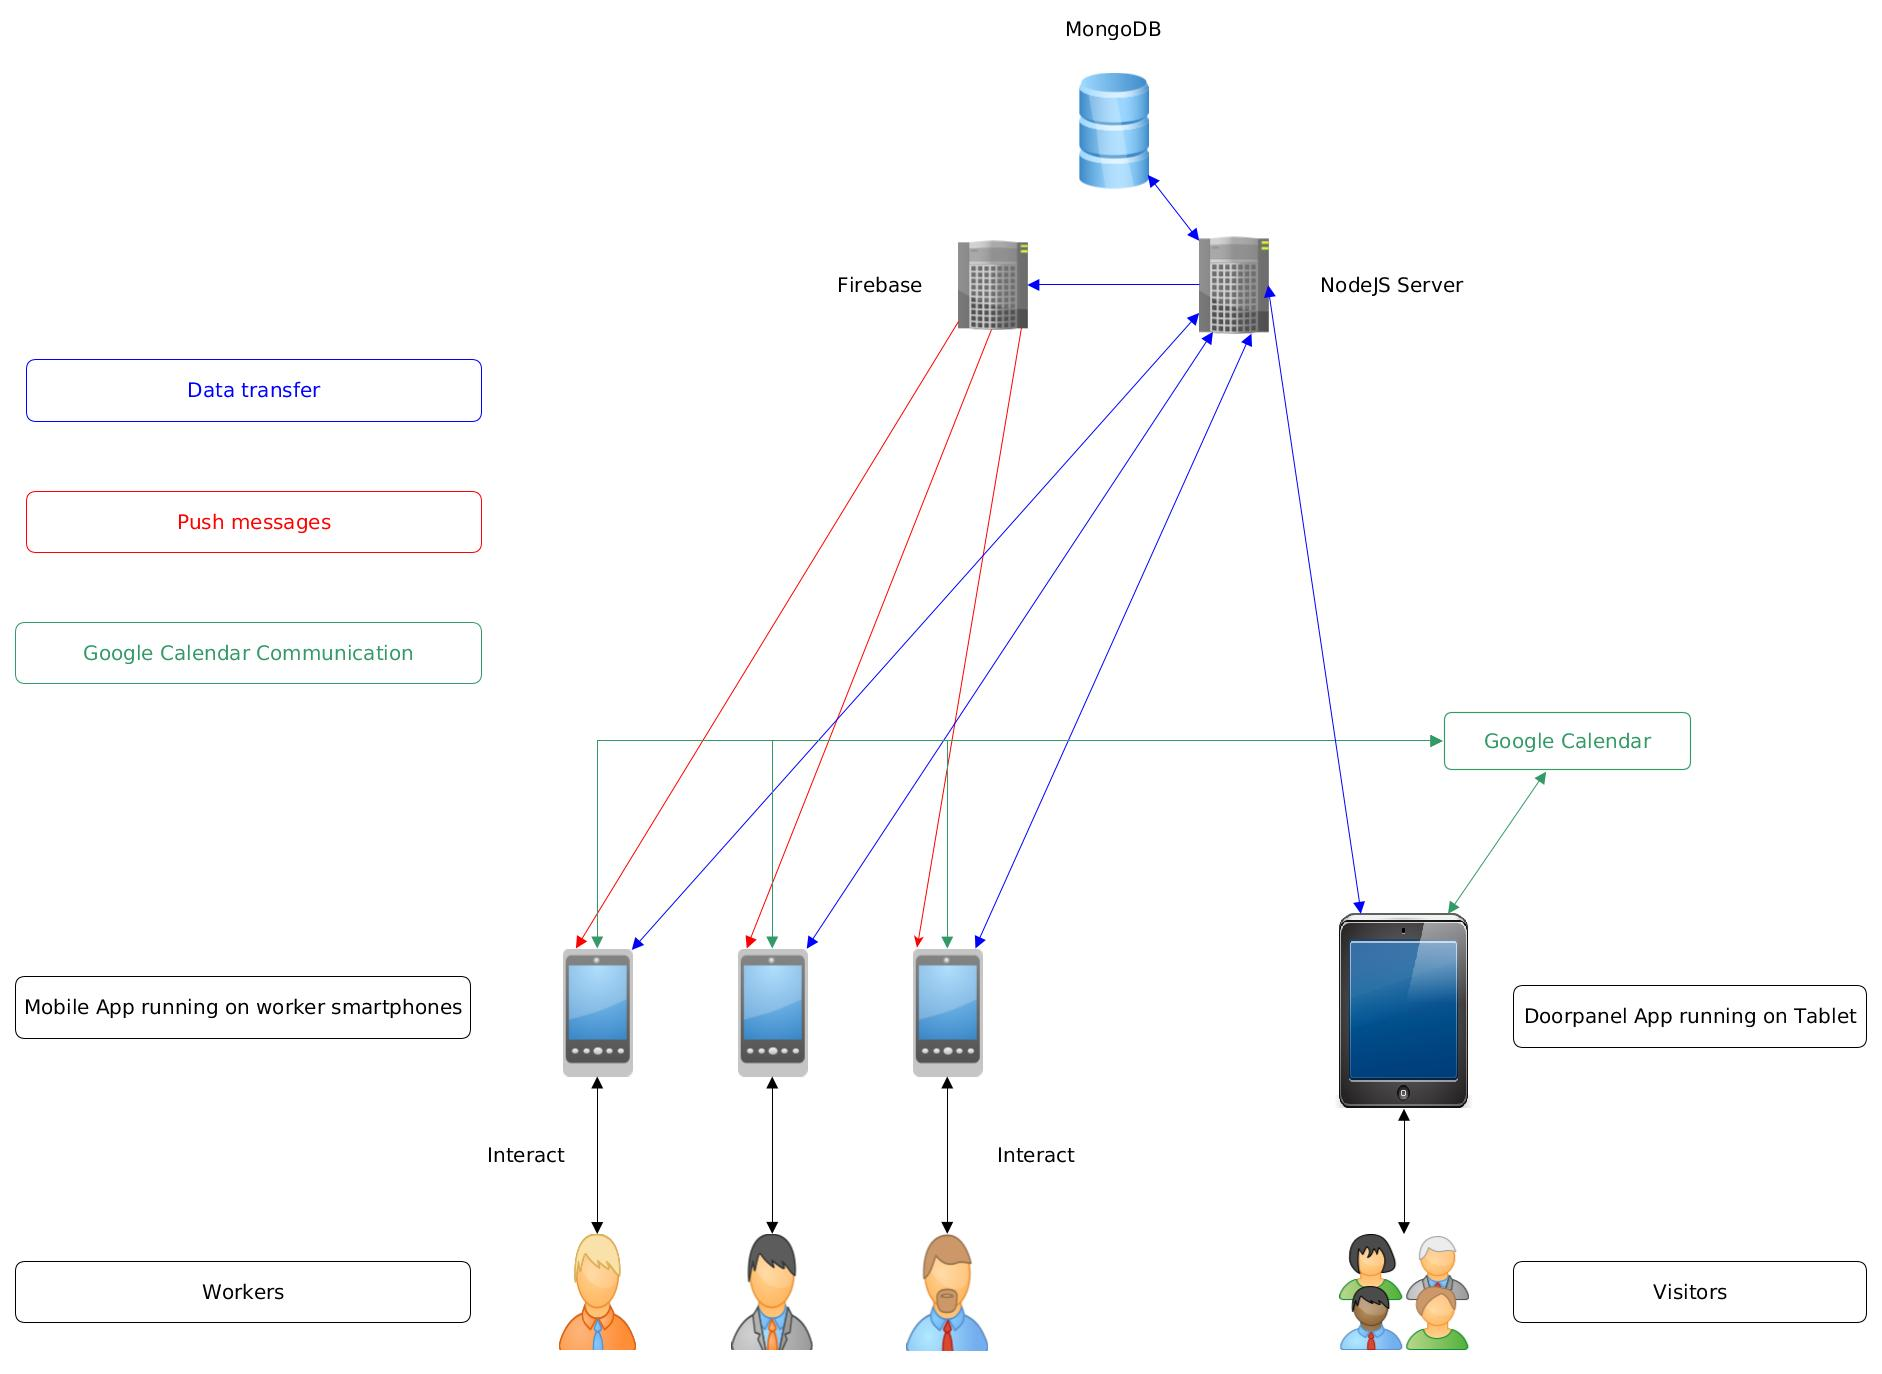
\includegraphics[max size={\textwidth}{\textheight}]{overview}
	    \caption[Structural overview]{Basic communication}
	 \end{figure}
	
	
	\subsection{Description of elements and their interaction}
	Lorerm ipsum
	
	
	\section{User Descripton}
	Lorem ipsum
	
	\subsection{Basic Funtionality}
	Lorem ipsum
	
	\subsection{Detailed explanation}
	\begin{figure}
	 \centering
	   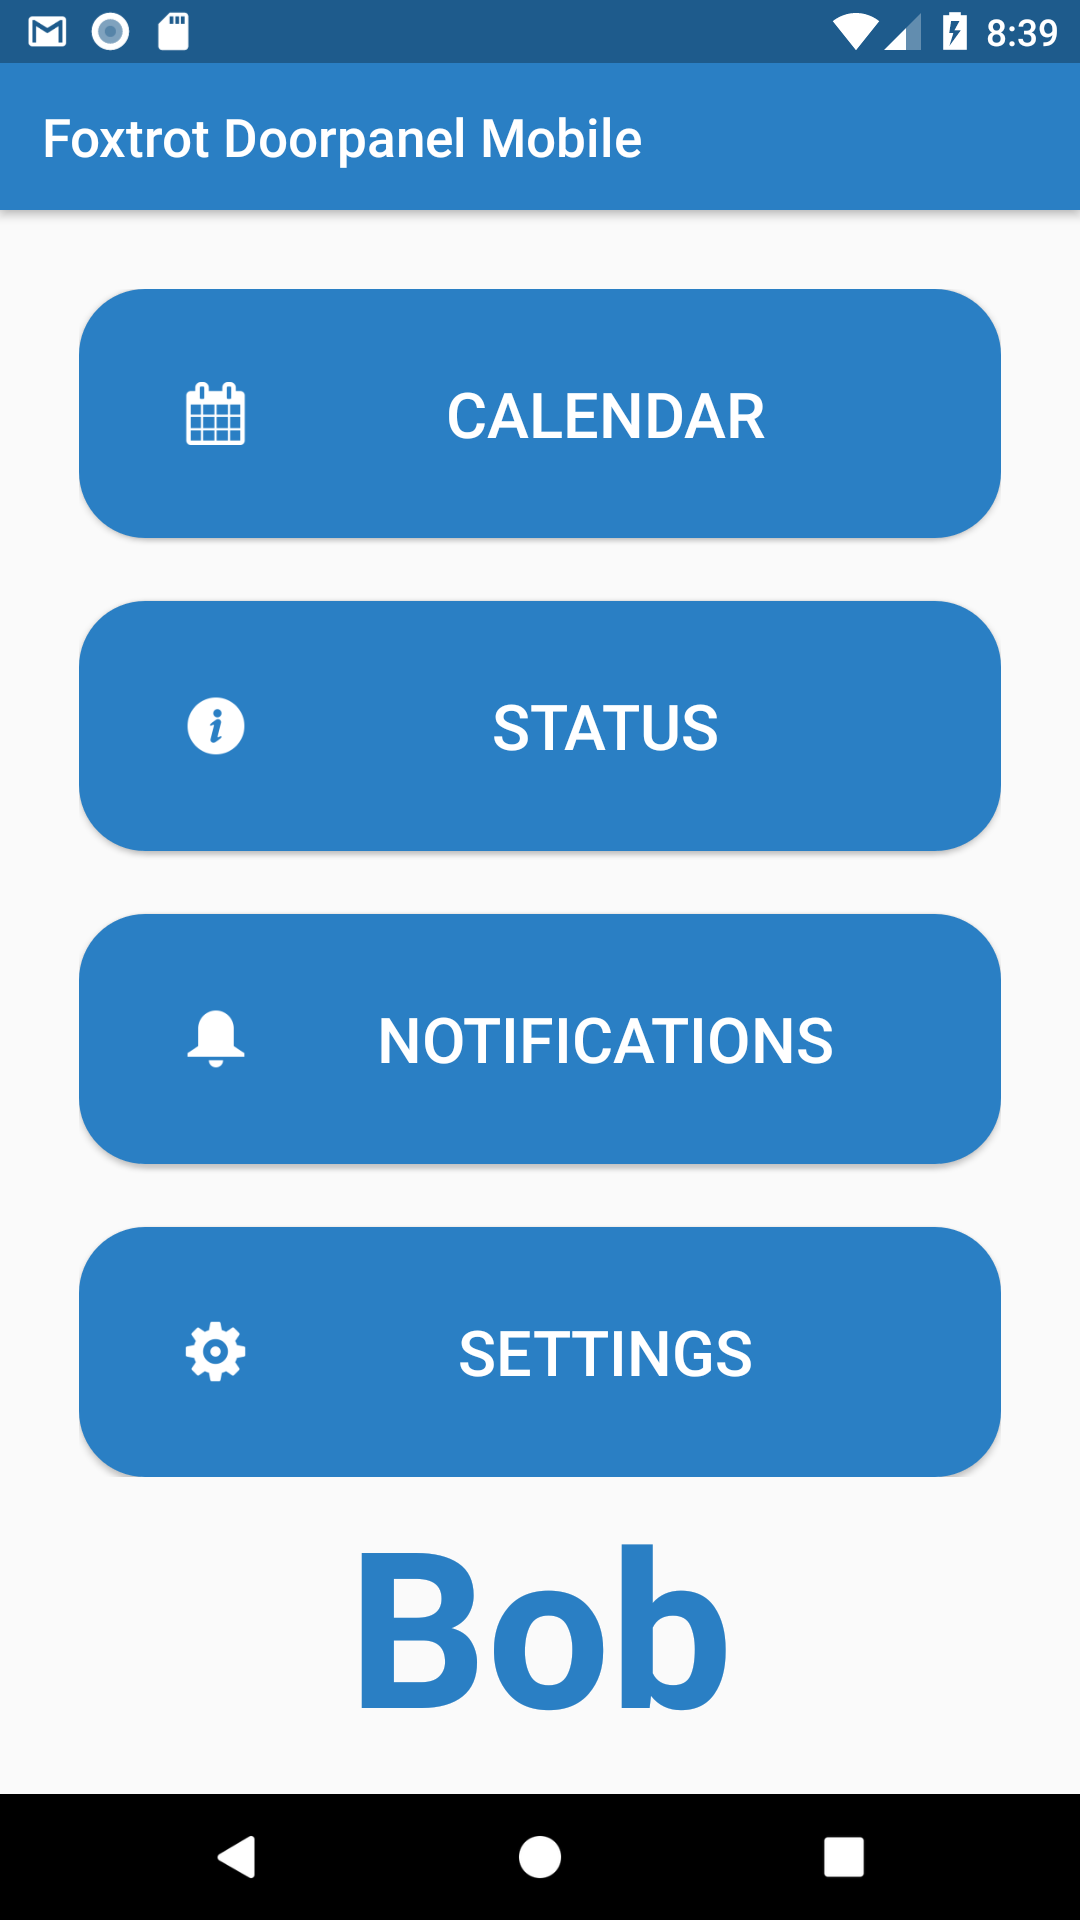
\includegraphics[width=30mm,scale=0.8]{mobile/Main-Screen.png}
	   \caption{Main Screen}
	\end{figure}

	\begin{figure}
		\centering
		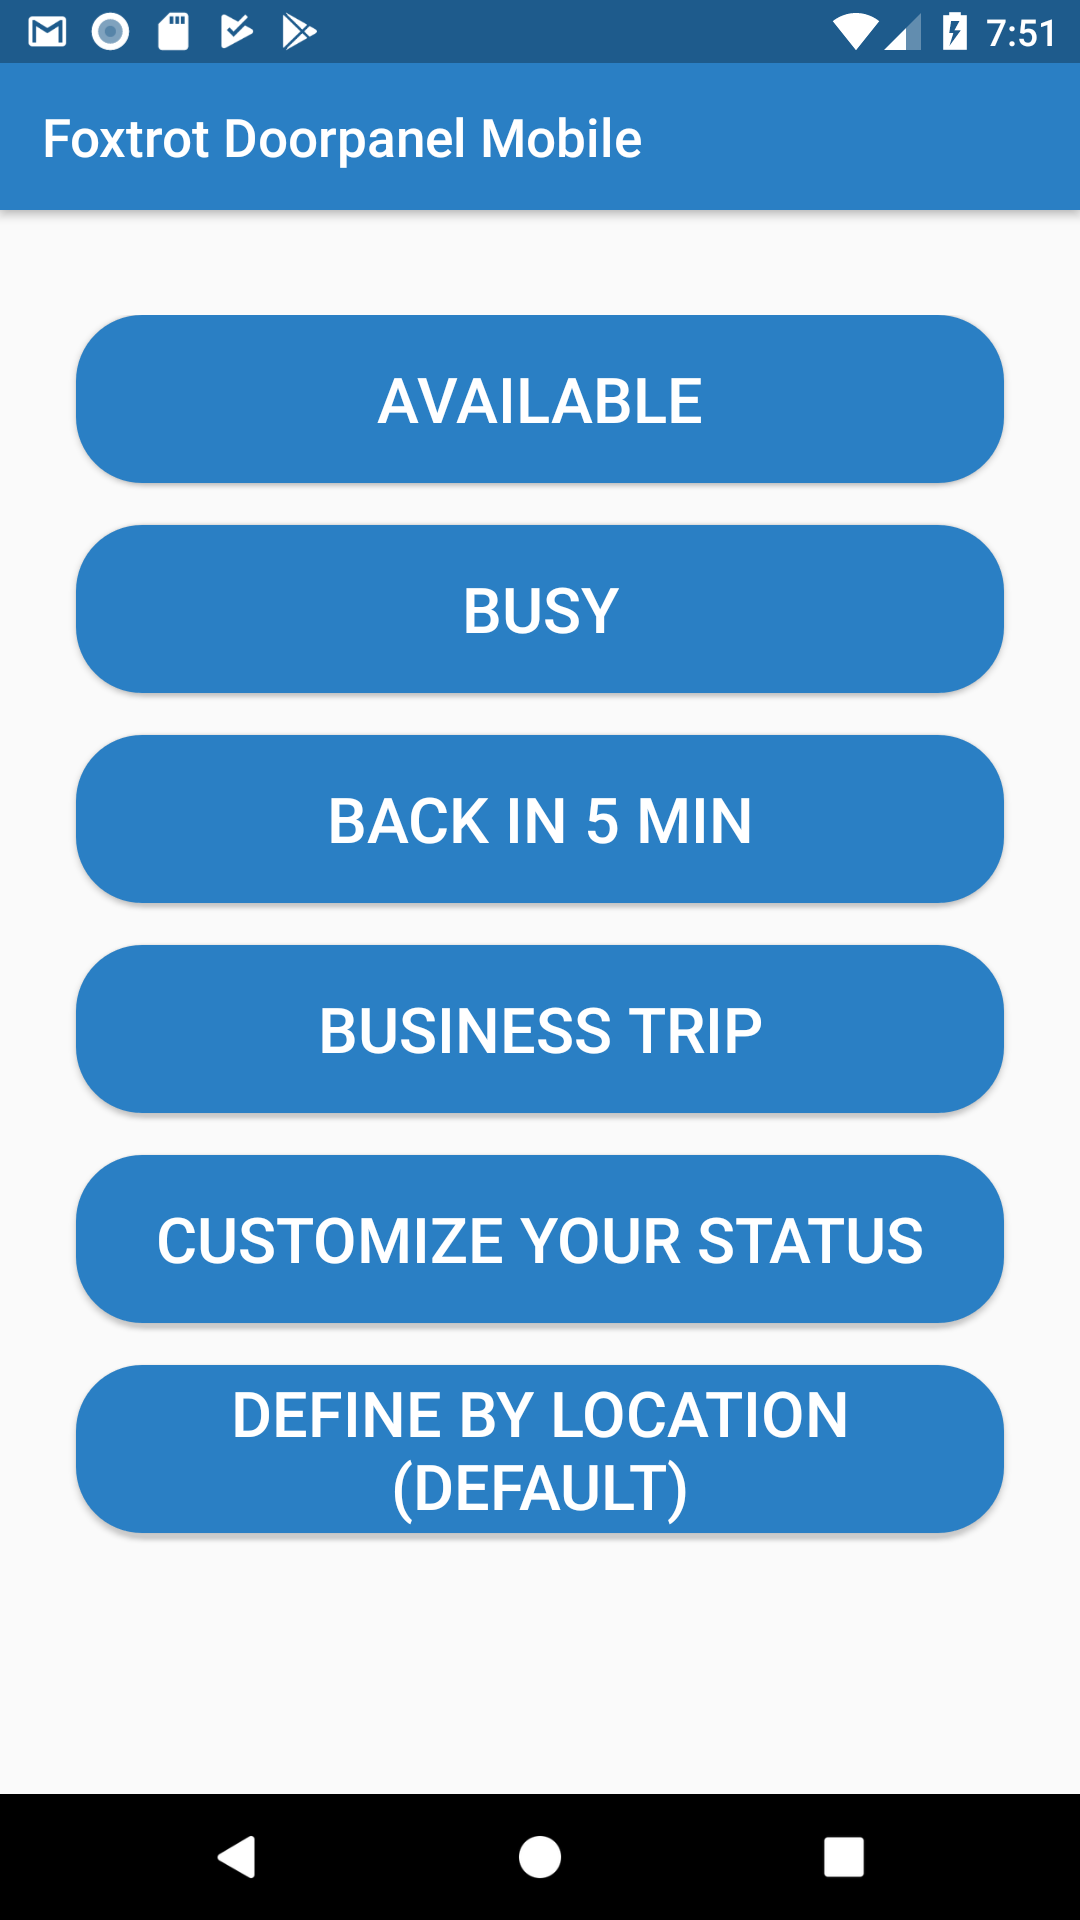
\includegraphics[width=30mm,scale=0.8]{mobile/Status-selection.png}
		\caption{Status Selection}
	\end{figure}

	\begin{figure}
		\centering
		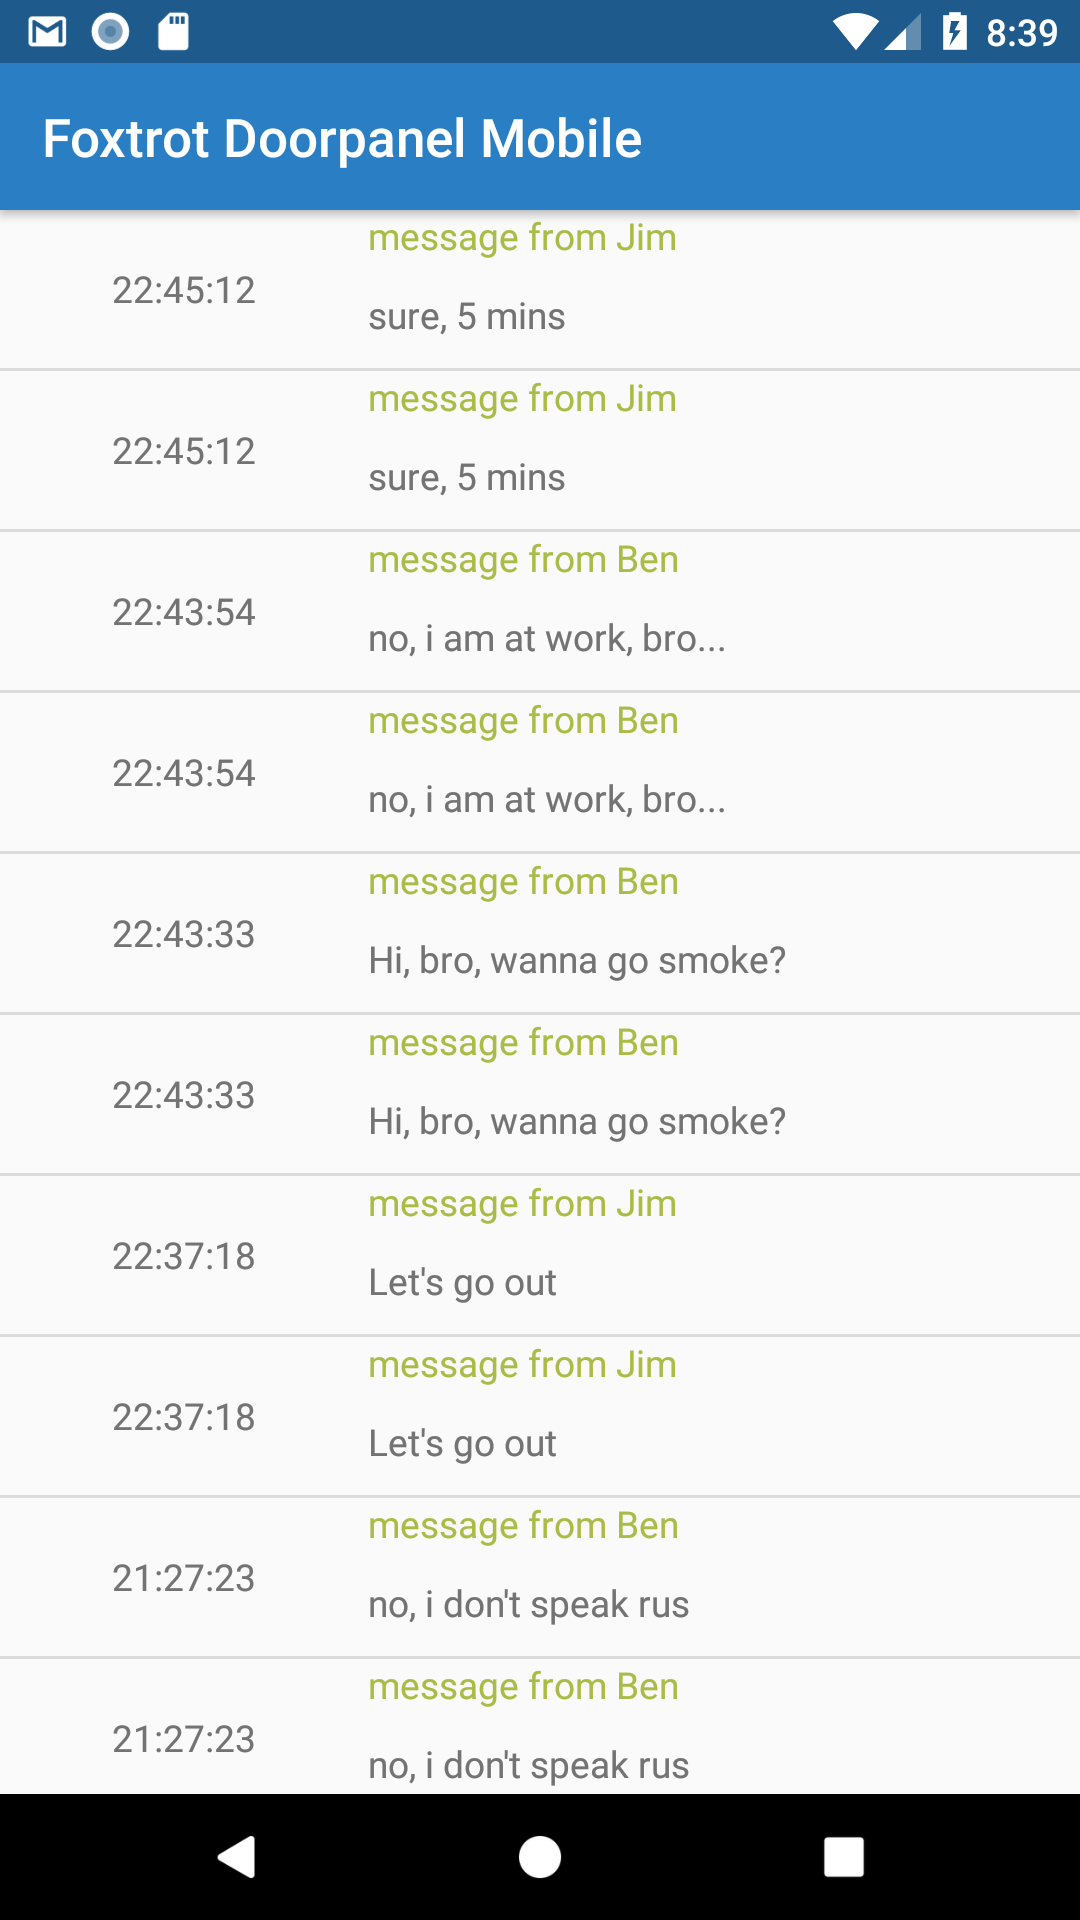
\includegraphics[width=30mm,scale=0.8]{mobile/Notifications.png}
		\caption{Notifications}
	\end{figure}

	\begin{figure}
		\centering
		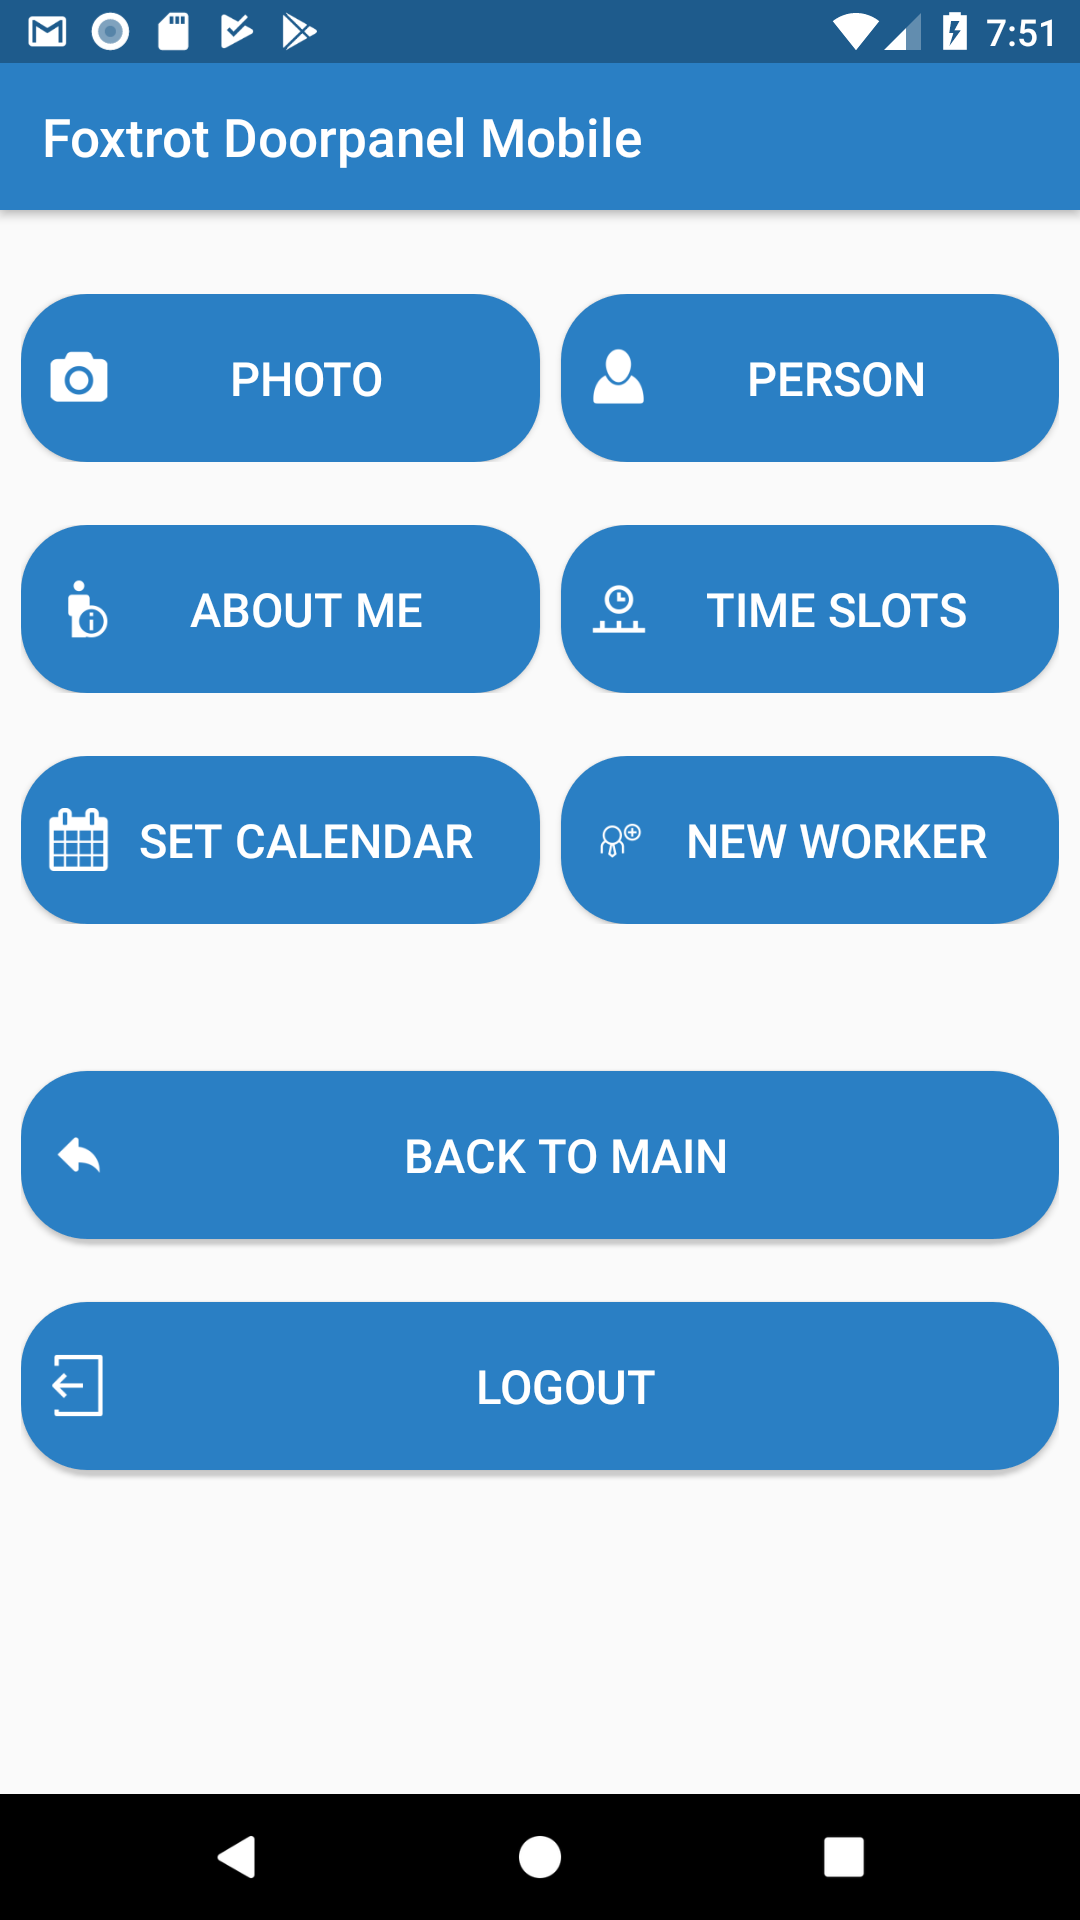
\includegraphics[width=30mm,scale=0.8]{mobile/Settings.png}
		\caption{Settings Main Level}
	\end{figure}	

	%
	Lorem ipsum.%
	%%\footnote{T.\ Pratchett: ''A guess? Well, that's good enough for physics!{``}}
	
	Lorem ipsum
	
	
	\listoffigures\addcontentsline{toc}{chapter}{\listfigurename}
\end{document}
